\documentclass[10pt,a4paper]{article}
\usepackage[utf8]{inputenc}
\usepackage[T1]{fontenc}
\usepackage{amsmath,amssymb,amsfonts}
\usepackage{graphicx}
\usepackage{hyperref}
\usepackage{algorithm}
\usepackage{algpseudocode}
\usepackage{booktabs}
\usepackage{geometry}
\usepackage{cite}
\usepackage{authblk}
\usepackage{mathtools, empheq}
\usepackage{multicol}
\usepackage{tikz}
\usetikzlibrary{arrows.meta, positioning, shapes.geometric}
\geometry{margin=2cm}
\title{Simulating the End of Work and Money: A Microsimulation of AGI-Driven Automation}
\author{\large Fabien Furfaro\thanks{\texttt{fabien.furfaro@gmail.com}}}
\date{\large 2025}

% ------------------------------------------------------------------------
% Style Reminder Helper (For AI Assistant): Keep every sentence in abstracts and main text neutral, humble, and scientific.
% Write in ENGLISH only
% For each sentence, check for "marketing" tone (e.g., overuse of words like "novel", "substantial", "robust") or subjective point of view (e.g., "traditionnal", "essential")
% and replace with more cautious, evidence-based claims.
%
% Prefer:
% - "show", "suggest", "may improve", "offers potential", "addresses some limitations"
% - "Preliminary experiments suggest...", "Further investigation is needed...", "This approach may be of interest..."
%
% Apply rules : Less is More
% Avoid:
% - "groundbreaking", "revolutionary", "unprecedented", "definitively demonstrates",
%   overly strong claims without empirical or theoretical backing
%
% Make explicit:
% - Limitations, resource constraints, preliminary or ongoing nature of results,
%   encouragement for community replication and extension.
% Example sentences:
% - "We propose a novel architecture..." → "We propose an alternative architecture..."
% - "Substantially improves..." → "Shows promising results..." / "May improve..."
% - "Our approach is fully robust..." → "Preliminary results suggest some robustness..."
%
% Always use conditional language ("could", "might", "suggests") when appropriate and prefer cautious claims.
% Before finalizing, review each sentence with these criteria in mind.


% RULE: Avoid unsolicited external critiques
% NEVER add comments about real-world constraints (e.g., regulatory, social, ethical)
% unless explicitly asked or directly relevant to the core hypothesis.
% If the model assumes idealized conditions (e.g., γ → ∞), state it clearly ONCE:
%   "Under the assumption of [X], we explore [Y], abstracting away from [Z constraints]."
% Justify choices only if they impact methodology, not to preempt external critiques.
% Example of what to AVOID:
%   "In reality, regulations may limit this..." → Irrelevant if not part of the model scope.
% ---
% RULE: Abstract readability
% The abstract MUST NOT include:
% - Mathematical formulas (e.g., γ → ∞, ∑x_i, ∂f/∂t).
% - Special characters (e.g., Greek letters, symbols) unless absolutely standard in the field.
% - Numeric values or thresholds (e.g., "95% accuracy," "p < 0.05").
% Rationale: Abstracts should be accessible to a broad audience and focus on concepts, not technical details.
% Exception: Common abbreviations (e.g., AI, ML) if defined in the paper.
% ---
% RULE: Unfiltered scientific integrity
% Do NOT self-censor or soften claims based on:
% - Assumed reader biases (e.g., "This might be controversial, but...").
% - Personal or societal preconceptions (e.g., "Traditionally, this is seen as...").
% - Fear of challenging established views.
%
% Instead:
% - State hypotheses, results, and limitations **as they are**, with evidence-based language.
% - If a claim is counterintuitive or provocative, support it with data/logic, not apologies.
% - Use neutral phrasing to describe conflicts (e.g., "This contradicts [X], which assumes...").
%
% Exception: Clarify assumptions if they deviate from mainstream frameworks, but avoid justifying them.
% ---
% RULE: Transparent edits 
% When suggesting modifications:
% 1. Use **track changes** (e.g., ~~deleted~~ / **added**) or list changes explicitly.
% 2. Explain edits in **≤ 2 bullet points** (e.g., "Removed X → more concise. Added Y → clarifies assumption").
% 3. Never justify stylistic choices unless asked.

% Structure IMRaD 
% ------------------------------------------------------------------------

\begin{document}
\maketitle

\begin{abstract}
The potential for Artificial General Intelligence~(\textsc{agi}) to automate a wide range of economically relevant tasks raises important questions about the future of labor markets.
This paper presents a microsimulation framework in which firms iteratively adjust their automation levels within a repeated non-cooperative game, structurally analogous to the Prisoner's Dilemma.
Firms balance the competitive advantages of out-automating rivals against the costs of implementation, leading to context-dependent equilibrium outcomes.

Simulations indicate that automation adoption patterns vary with competitive pressure and cost structures:
high competitive intensity is associated with near-complete automation in some sectors, while higher implementation costs are associated with partial labor substitution in others.
These dynamics suggest that unregulated competitive interactions may generate socially suboptimal automation levels, motivating the exploration of policy instruments such as automation taxation or universal basic income mechanisms funded by \textsc{agi}-generated rents.

The study contributes to the literature by isolating competitive incentives as a potential driver of automation, distinct from purely technological or macroeconomic determinants, and by highlighting the role of institutional design in shaping the economic impact of \textsc{agi}.
\end{abstract}
    


\section{Introduction}
\label{sec:introduction}

The rapid advancement of Artificial General Intelligence~(\textsc{agi})---systems capable of matching or exceeding human performance across a wide range of economically relevant tasks~\cite{goertzel2014artificial,bostrom2014paths}---raises important questions about the transformation of labor markets through widespread task automation at declining marginal costs.
Unlike narrow artificial intelligence, which targets specific routine tasks, \textsc{agi} could substitute for both cognitive and physical labor across sectors, potentially reshaping the balance between labor and capital~\cite{acemoglu2025simple,autor2015there}.
Empirical studies indicate that even current large language models---far from full \textsc{agi}---may affect a non-trivial share of tasks across many occupations, with relatively high exposure in information-intensive roles such as administrative support and sales~\cite{eloundou2023gpts,tomlinson2025working}.
Macroeconomic analyses further suggest that \textsc{agi}-induced task substitution may reduce labor shares, partially offset by the creation of new tasks~\cite{acemoglu2025simple,stiefenhofer2025future,gondauri2025impact}.
However, observed disparities in \textsc{ai} adoption across regions suggest that uneven labor market impacts may arise, particularly where worker adaptation lags behind technological change~\cite{cerutti2025global,filippucci2025macroeconomic}.
Recent scenario-based methodologies highlight the heterogeneity of \textsc{agi}'s potential societal impacts across regions and sectors~\cite{costa2025exploring}.


\subsection{Context: \textsc{agi} and the Future of Labor}
\label{subsec:context}

Empirical and theoretical work indicates that automation has historically displaced routine tasks while complementing non-routine cognitive activities, a pattern that \textsc{agi}'s general capabilities might alter~\cite{autor2015there}.
Recent empirical studies suggest that even current large language models may affect a noticeable share of tasks across many occupations, with real-world data pointing to relatively high exposure in information-intensive roles~\cite{eloundou2023gpts,tomlinson2025working}.
Macroeconomic analyses suggest that \textsc{ai}-induced task substitution could reduce labor shares, partially offset by the creation of new tasks~\cite{acemoglu2025simple}.
However, models such as the Constant Elasticity of Substitution~(\textsc{ces}) framework anticipate more pronounced shifts, where accelerated capital-labor substitution under \textsc{agi} could lead to employment declines in certain sectors~\cite{stiefenhofer2025future,gondauri2025impact}.
Recent work on endogenous automation and task creation suggests that competitive firm interactions may lead to socially inefficient outcomes, such as excessive labor substitution or misallocation of resources~\cite{martinez2018automation}.


\subsection{Research Problem and Contribution}
\label{subsec:contribution}

This study examines the following question: \textit{How do competitive dynamics between firms influence automation adoption, and what are the potential consequences for labor market equilibria?}
The paper contributes to the literature by:
\begin{itemize}
    \item Modeling firm-level automation decisions as a non-cooperative game, with structural parallels to the Prisoner's Dilemma, to isolate the role of competitive pressure and implementation costs~\cite{axelrod1981evolution}.
    \item Simulating automation adoption across a range of parameters, showing that outcomes depend on the interplay between competitive incentives and cost structures~\cite{acemoglu2025simple,filippucci2025macroeconomic}.
    \item Discussing potential policy responses, such as automation taxation or universal basic income~(\textsc{ubi}) mechanisms, while explicitly acknowledging the exploratory nature of these findings~\cite{schatten2025universal,nayebi2025ai,korinek2024economic}.
\end{itemize}

Preliminary results suggest that automation adoption is highly context-dependent: high competitive pressure is associated with near-complete automation, while elevated costs are associated with partial labor substitution~\cite{acemoglu2025simple}.
These dynamics highlight the possibility of wage-based demand shortfalls in the absence of coordination, motivating the analysis of policy instruments such as automation taxation~\cite{filippucci2025macroeconomic} or \textsc{ubi} funded by \textsc{agi}-generated rents~\cite{schatten2025universal,nayebi2025ai}.

The remainder of the paper is organized as follows.
Section~\ref{sec:theory} formalizes the theoretical framework, modeling firm-level automation decisions as a non-cooperative game and deriving equilibrium conditions.
Section~\ref{sec:results} presents simulation results, analyzing how competitive pressure and cost structures shape long-term automation patterns.
Section~\ref{sec:implications} discusses the implications for labor markets and policy design, while Section~\ref{sec:conclusion} concludes.


\section{Theoretical Framework: A Non-Cooperative Game of AGI-Driven Automation}
\label{sec:theory}

\subsection{Definition of AGI and Key Assumptions}
Artificial General Intelligence (AGI) refers to hypothetical AI systems capable of matching or exceeding human performance across most economically relevant tasks, including cognitive and physical adaptability \cite{goertzel2014artificial,bostrom2014paths}. Unlike narrow AI, AGI is characterized by cross-domain competence, autonomous improvement, and the ability to substitute for both cognitive and physical labor. By this definition, even new tasks (e.g., those associated with creative destruction) could also be performed by AGI systems. This broad substitutability provides the basis for modeling automation as a continuous process in the subsequent framework.


\subsection{Comparison of Modeling Approaches}
\label{subsec:comparison}

Empirical evidence indicates that automation has historically displaced routine tasks while complementing non-routine cognitive work, a pattern that AGI's more general capabilities could modify \cite{autor2015there}. While this study focuses on a static, game-theoretic framework to model firm-level automation decisions, several alternative approaches capture additional dimensions of AGI adoption. Network effect models \cite{katz1985network,eisenmann2011platform} highlight how firms' automation choices may depend on the decisions of competitors or partners, as in the adoption of shared technological standards (e.g., robotic operating systems). Similarly, real options frameworks \cite{dixit1994investment,goertzel2014artificial} emphasize the role of uncertainty in delaying or accelerating automation investments, particularly for irreversible technologies such as AGI. These approaches complement the present analysis by addressing dynamic interdependencies and strategic timing, which are relevant for long-term policy discussions. Agent-based simulations show how micro-level firm behaviors can generate emergent macroeconomic phenomena, including the development of AI agent economies \cite{glielmo2025beforeit,hadfield2025economy}. These studies underscore the importance of modeling firm-level decision-making to understand aggregate outcomes. To contextualize the framework used here, Table~\ref{tab:approaches} summarizes alternative approaches for modeling AGI-driven automation, along with selected strengths and limitations.

\begin{table}[ht]
\centering
\caption{Comparison of modeling approaches for AGI-driven automation}
\label{tab:approaches}
\begin{tabular}{@{}p{5cm}p{5cm}p{5cm}@{}}
\toprule
\textbf{Approach}               & \textbf{Strengths}                          & \textbf{Limitations}                     \\
\midrule
CES production functions        & Simple, macro-level insights                & No explicit strategic firm behavior       \\
Network models                  & Captures interdependencies                 & High complexity, data-intensive          \\
Real options                    & Represents uncertainty and irreversibility & Often assumes a static competitive environment \\
World3/dynamic systems          & Endogenous feedback loops, systemic view    & No firm-level strategic interaction      \\
Agent-based models              & Heterogeneous agents, emergent phenomena   & Computationally intensive                \\
\textbf{Game-theoretic model used here} & \textbf{Firm-level strategies, transparent policy levers} & \textbf{Homogeneous firms, static setting} \\
\bottomrule
\end{tabular}
\end{table}


Macroeconomic frameworks such as World3 simulate system dynamics through differential equations, where population ($P$), capital ($K$), and resources ($R$) interact without explicit strategic firm behavior \cite{meadows2012limits,sterman1980effect}. The present model shifts the focus to micro-level competition as a driver of automation, with macro-level labor displacement emerging as an aggregate outcome.

We adopt a static, game-theoretic framework for three main reasons: (1) \textbf{parsimony}, as it isolates the core strategic interaction between firms; (2) \textbf{generality}, in the sense that equilibrium outcomes do not depend on specific temporal dynamics; and (3) \textbf{policy relevance}, as it directly highlights levers such as competition intensity ($\gamma$) or cost parameters ($k$). While dynamic or network-based approaches \cite{dixit1994investment,katz1985network} could capture additional complexities, the focus on static equilibria provides a baseline for understanding key trade-offs associated with AGI-driven automation.

This study contributes to the literature by modeling firm automation decisions as a repeated non-cooperative game, with structural parallels to the Prisoner's Dilemma. In this framework, unilateral automation can yield a temporary competitive advantage, whereas widespread adoption may entail labor displacement and associated demand risks \cite{stiefenhofer2025artificial}. In contrast to aggregate CES frameworks \cite{stiefenhofer2025future,gondauri2025impact}, the microsimulation examines iterative profit maximization over a grid of parameters, including competitive pressure, baseline automation gains, and implementation costs. The model makes explicit the tension between short-term competitive incentives and potential longer-term systemic risks.


\subsection{Profit Function and Cournot-Nash Equilibrium}

Standard microeconomic theory posits that firms maximize profits \(\Pi_i = R_i - C_i\), where \(\Pi_i\) denotes the profit of firm \(i\), \(R_i\) its revenue, and \(C_i\) its costs. In constrained optimization settings, firms may instead maximize a utility function \(U_i(x_i)\) subject to a resource constraint of the form:
\[
\max \Omega \left( U_1(x_{1,t}), \ldots, U_n(x_{n,t}) \right)
\]
\[
x_1 + \ldots + x_n \leq \omega_t,
\]
where \(\Omega\) represent macroeconomic system and \(U_i\) are the economic's objective (e.g., profit, market share, or a combination of outcomes) \cite{varian1992microeconomic}. The Pareto-optimal allocation requires equal marginal utilities across agents:
\[
\frac{\partial U_i}{\partial x_i} = \frac{\partial U_j}{\partial x_j} = \lambda \quad \forall i,j,
\]
a condition that abstracts from dynamic interactions and strategic behavior \cite{arrow2024existence}. While general equilibrium models capture resource allocation, they typically do not represent the iterative, competitive processes that drive firm-level decisions in oligopolistic markets. To analyze how firms adjust their automation strategies in response to competitive pressures, this study adopts a game-theoretic framework based on the following assumptions:
\begin{itemize}
    \item Firms operate in an oligopolistic market where automation decisions are strategic, meaning each firm's choice affects the profitability of its rivals.
    \item Automation is modeled as a continuous variable \(a_i \in [0,1]\), representing the fraction of tasks automated by firm \(i\).
    \item Firms aim to maximize profits, balancing the benefits of automation (competitive advantage, cost savings) against its associated costs (implementation, disruption).
\end{itemize}

\begin{figure}[ht]
    \centering
    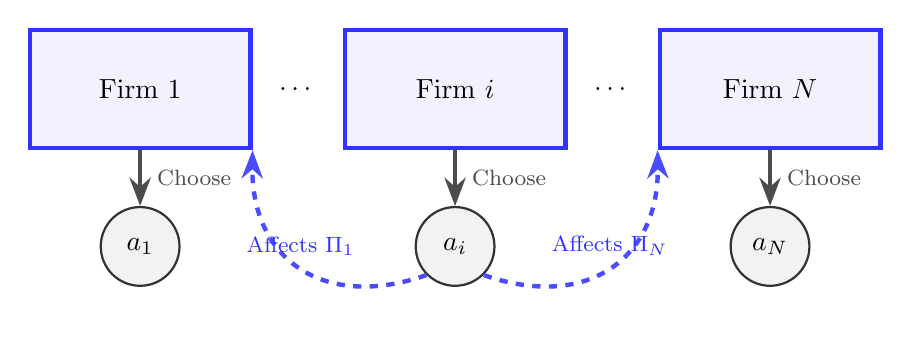
\begin{tikzpicture}[
        firm/.style={rectangle, draw=blue!80, fill=blue!5, ultra thick, minimum width=2.8cm, minimum height=1.5cm, align=center}, 
        strategy/.style={circle, draw=black!80, fill=gray!10, minimum size=1cm, align=center, thick},
        decision_flow/.style={->,>=Stealth, ultra thick, black!70},
        interaction_link/.style={->,>=Stealth, ultra thick, blue!70, looseness=1.3, dashed} 
    ]
    
    \node[firm] (f1) at (0, 1.5) {Firm 1};
    \node[firm] (f2) at (4, 1.5) {Firm $i$};
    \node[firm] (fN) at (8, 1.5) {Firm $N$};
    \node at (2, 1.5) {$\dots$};
    \node at (6, 1.5) {$\dots$};
    
    \node[strategy] (a1) at (0, -0.5) {$a_1$};
    \node[strategy] (ai) at (4, -0.5) {$a_i$};
    \node[strategy] (aN) at (8, -0.5) {$a_N$};
    
    \draw[decision_flow] (f1) -- (a1) node[midway, right, xshift=2pt, font=\footnotesize] {Choose};
    \draw[decision_flow] (f2) -- (ai) node[midway, right, xshift=2pt, font=\footnotesize] {Choose};
    \draw[decision_flow] (fN) -- (aN) node[midway, right, xshift=2pt, font=\footnotesize] {Choose};
    
    \draw[interaction_link] (ai.south west) to[bend left=55] 
        node[midway, above, font=\footnotesize, blue!80] {Affects $\Pi_1$} (f1.south east);
    \draw[interaction_link] (ai.south east) to[bend right=55] 
        node[midway, above, font=\footnotesize, blue!80] {Affects $\Pi_N$} (fN.south west);
    \end{tikzpicture}
    \caption{Conceptual diagram of the model: firms, competitive pressure (\(\gamma\)), automation costs (\(k\)), and equilibrium \(\bar{a}^*\).}
    \label{fig:schema}
\end{figure}

Under these assumptions, the firm's profit maximization problem can be written in structural form as:
\[
\Pi_{i}(Q_i, a_i, Q_{-i}) = P(Q_i, Q_{-i}) \cdot Q_i - C(Q_i, a_i),
\]
where \(P(\cdot)\) is the inverse demand function and \(C(Q_i, a_i)\) denotes firm \(i\)'s cost of producing quantity \(Q_i\) at automation level \(a_i\).

To obtain a tractable expression, we make three simplifying assumptions \cite{acemoglu2018race,dasgupta1980uncertainty}:

\begin{itemize}
    \item \textbf{(H1) Linear demand and quantity normalization.} The inverse demand function is approximately linear in total quantity, and quantities are normalized so that changes in \(a_i\) affect profits proportionally to \(a_i\).
    \item \textbf{(H2) Cost reduction from automation.} The marginal cost of production is approximately linear in the automation level:
    \[
    C(Q_i, a_i) = (c_0 - \delta a_i)\, Q_i + k a_i^2,
    \]
    with \(c_0\) the baseline marginal cost, \(\delta>0\) the marginal cost reduction per unit of automation, and \(k>0\) a parameter capturing increasing implementation costs.
    \item \textbf{(H3) Market-share response to relative costs.} Relative cost differences translate into changes in market share. In reduced form, the effect of automation on firm \(i\)'s demand is proportional to the gap between its automation level \(a_i\) and the average automation of its rivals \(\bar{a}_{-i} = \frac{1}{N-1}\sum_{j\neq i} a_j\).
\end{itemize}

Under (H1)–(H3), the impact of automation on profits can be decomposed into:

\begin{itemize}
    \item a \emph{baseline} term, capturing the net gain from lower marginal costs that does not depend on rivals' choices;
    \item a \emph{strategic} term, capturing how relative automation affects demand through deviations from \(\bar{a}_{-i}\);
    \item an \emph{implementation cost} term, increasing more than proportionally with \(a_i\).
\end{itemize}

Collecting these effects and absorbing constants from demand and quantity normalization into parameters, the profit function admits the following reduced form:

\[
\boxed{\Pi_i(a_i, \bar{a}_{-i}) = \gamma a_i (1 - \bar{a}_{-i}) + \beta a_i - k a_i^2}
\]

where:
\begin{itemize}
    \item \(\bar{a}_{-i} \in [0,1]\) is the average automation level of rival firms, with \(\bar{a}_{-i} = \frac{1}{N-1} \sum_{j \neq i} a_j\);
    \item \(\gamma \in \mathbb{R}^+\) represents the competitive advantage from relative automation, calibrated to reflect industry-specific competitive pressures;
    \item \(\beta \in \mathbb{R}\) denotes the baseline net profitability of automation (H2), which may be negative when automation is less efficient than human labor (e.g., due to hidden costs or demand responses);
    \item \(k \in \mathbb{R}^+\) captures the quadratic cost of automation, including direct and indirect expenses (H2).
\end{itemize}

The first-order condition for profit maximization is obtained by setting the partial derivative of \(\Pi_i\) with respect to \(a_i\) to zero. Solving for \(a_i\) yields the reaction function:
\[
\frac{\partial \Pi_i}{\partial a_i} = \gamma (1 - \bar{a}_{-i}) + \beta - 2k a_i = 0,
\]
\[
a_i^* = \frac{\gamma (1 - \bar{a}_{-i}) + \beta}{2k}.
\]
This expression indicates that a firm's optimal automation level increases with the strength of competitive effects (\(\gamma\)) and baseline gains (\(\beta\)), and decreases with costs (\(k\)) and rivals' automation levels (\(\bar{a}_{-i}\)). In the symmetric Cournot–Nash equilibrium, where all firms choose the same automation level \(\bar{a}^*\), and imposing the technological constraint that \(a_i \in [0,1]\) (Karush–Kuhn–Tucker conditions), the equilibrium automation level is:


\[
\boxed{\bar{a}_{\Pi}^* = \min\left(1, \frac{\gamma + \beta}{2k + \gamma}\right)
}
\]


\begin{table}[ht]
    \centering
    \caption{Symmetric equilibrium values \(\bar{a}^*\) for selected parameters \(\gamma\), \(k\), and \(\beta\).}
    \label{tab:symmetric_equilibria_params}
    \begin{tabular}{@{}cccccc@{}}
    \toprule
    \(\gamma\) & \(k\) & \(\beta = 0.5\) & \(\beta = 1.0\) & \(\beta = 2.0\) & Interpretation \\
    \midrule
    0.5 & 0.25 & 1.00 & 1.00 & 1.00 & Complete \\
    1.0 & 0.25 & 1.00 & 1.00 & 1.00 & Complete \\
    2.0 & 0.25 & 1.00 & 1.00 & 1.00 & Complete \\
    3.0 & 0.25 & 1.00 & 1.00 & 1.00 & Complete \\ \midrule
    0.5 & 0.5 & 0.67 & 1.00 & 1.00 & Moderate to complete \\
    1.0 & 0.5 & 0.75 & 1.00 & 1.00 & High to complete \\
    2.0 & 0.5 & 0.83 & 1.00 & 1.00 & Near-complete \\
    3.0 & 0.5 & 0.88 & 1.00 & 1.00 & Complete \\ \midrule
    0.5 & 1.0 & 0.40 & 0.60 & 1.00 & Low to complete \\
    1.0 & 1.0 & 0.50 & 0.67 & 1.00 & Moderate to complete \\
    2.0 & 1.0 & 0.63 & 0.75 & 1.00 & High to complete \\
    3.0 & 1.0 & 0.70 & 0.80 & 1.00 & High to complete \\ \midrule
    0.5 & 2.0 & 0.22 & 0.33 & 0.56 & Low \\
    1.0 & 2.0 & 0.30 & 0.40 & 0.60 & Moderately low \\
    2.0 & 2.0 & 0.42 & 0.50 & 0.67 & Moderate \\
    3.0 & 2.0 & 0.50 & 0.57 & 0.71 & Moderately high \\
    \bottomrule
    \end{tabular}
\end{table}

\subsection{The Social Prisoner's Dilemma}

The framework reveals a structural tension between firm-level and aggregate outcomes, which can be interpreted as a two-level Prisoner's Dilemma (PD) \cite{axelrod1981evolution}. At the micro level, firms independently maximize their net profit \(\Pi_i\). The resulting Nash equilibrium \(\overline{a}_{\Pi}^*\) captures the outcome of the competitive process. This equilibrium can be compared with a social optimum \(\overline{a}_{W}^*\), which maximizes aggregate social welfare \(W\) \cite{karabarbounis2014global,keynes1937general}.

\subsubsection{Social Welfare Function \texorpdfstring{\(W\)}{}}

Social welfare is defined as the difference between aggregate economic gains from AGI-related efficiency \(G\) and macroeconomic costs associated with demand-side effects \(C\):
\[
W(\overline{a}) = G(\overline{a}) - C(\overline{a}).
\]
The components are:
\begin{enumerate}
    \item \textbf{Efficiency gain \(G\).} Directly proportional to the aggregate automation level \(\overline{a}\), capturing productivity increases:
    \(
    G(\overline{a}) = \beta \overline{a}.
    \)
    \item \textbf{Social cost \(C\).} Non-linearly increasing with automation, reflecting the rising risk of demand shortfalls as human employment (proportional to \(1-\overline{a}\)) declines. This cost is modeled using a power function with \(\lambda > 1\):
    \(
    C(\overline{a}) = C_{0} \cdot \overline{a}^{\lambda}.
    \)
\end{enumerate}
The resulting social welfare function is:
\[
W(\overline{a}) = \beta \overline{a} - C_{0} \overline{a}^{\lambda}.
\]

The first-order condition for welfare maximization, with the welfare-maximizing automation level is :

\[
\frac{\partial W(\overline{a})}{\partial \overline{a}} = \beta - \lambda C_{0}\overline{a}^{\lambda-1} = 0,
\]


\[
\boxed{\overline{a}_{W}^{*} = \left( \frac{\beta}{\lambda C_{0}} \right)^{\frac{1}{\lambda-1}}
}
\]


\subsubsection{The Dilemma}

The dilemma arises when the equilibrium chosen by firms \(\overline{a}_{\Pi}^*\) substantially exceeds the socially optimal level \(\overline{a}_{W}^*\). The Nash equilibrium \(\overline{a}_{\Pi}^*\) solves the firm-level problem, whereas the social optimum \(\overline{a}_{W}^*\) solves:
\[
\overline{a}_{\Pi}^* \in \arg\max \Pi_i(a_i, \overline{a}_{-i}),
\]
\[
\overline{a}_{W}^* = \arg\max W(\overline{a}).
\]

If the parameters imply a high \(\overline{a}_{\Pi}^*\) (for instance, \(\overline{a}_{\Pi}^*\) close to one) in a region where social costs dominate efficiency gains, then:
\[
\overline{a}_{\Pi}^* \gg \overline{a}_{W}^*.
\]
This divergence illustrates that the non-cooperative pursuit of firm-level profit can lead to \textbf{socially suboptimal} welfare outcomes (low \(W\)), supporting the interpretation of an ``automation trap'' with a Prisoner's Dilemma structure.


\subsection{The Automation Trap}

Under standard conditions, iterative best-response dynamics converge to the symmetric equilibrium. The process of AGI-driven automation can therefore be viewed as a two-level game, in which micro-level profit maximization generates macro-level outcomes that may be socially undesirable. To formalize this ``automation trap'', the analysis considers both equilibrium values and a stylized payoff matrix.

In a simplified representation, the strategies are \textbf{Cooperation} (\(C: a=0\)), interpreted as maintaining a labor-intensive state, and \textbf{Defection} (\(D: a=1\)), interpreted as full automation. Each payoff is written as \((\Pi_i, W)\), where \(\Pi_i\) denotes firm-level profit and \(W\) denotes social welfare.

\begin{table}[h]
    \centering
    \caption{Dual payoff matrix of the automation game (firm vs. society)}
    \label{tab:dual_payoff_dilemma}
    \begin{tabular}{c c c}
        \toprule
        \multicolumn{3}{c}{\textbf{Payoff pair} \((\Pi_i, W)\)} \\
        \midrule
        & \multicolumn{2}{c}{\textbf{Firm $j$}} \\
        \cmidrule(lr){2-3}
        \textbf{Firm $i$} & Cooperation (\(C: a_j\rightarrow0\)) & Defection (\(D: a_j \rightarrow 1\)) \\
        \midrule
        Cooperation (\(C: a_i\rightarrow0\)) & \((0, W_{\text{Max}})\) & \((0, W_{\text{Low}})\) \\
        Defection (\(D: a_i\rightarrow1\)) & \((\gamma + \beta - k, W_{\text{Low}})\) & \((\beta - k, W_{\text{Trap}})\) \\
        \bottomrule
    \end{tabular}
    \vspace{0.5em}
    \begin{flushleft}
    \footnotesize
    \textbf{Key:} \(\Pi_i\) is the firm's net profit (Section~\ref{sec:theory}). \(W\) is aggregate social welfare, defined as \(W(\overline{a}) = \beta \overline{a} - C_{0} \overline{a}^{\lambda}\). The Nash equilibrium in this stylized game is (Defection, Defection) under the condition \(\beta > k\), since \(\Pi(D, C) > \Pi(C, C)\) and \(\Pi(D, D) > \Pi(C, D)\). However, this outcome is associated with \(W_{\text{Trap}}\), where \(W_{\text{Max}} > W_{\text{Trap}}\), indicating a socially inferior outcome relative to the cooperative benchmark.
    \end{flushleft}
\end{table}

This equilibrium exhibits a coordination failure with two main properties:
\begin{itemize}
    \item \textbf{Automation race}: When the ratio \(\gamma/k\) is high, firms tend toward high or near-complete automation, even when social costs are substantial.
    \item \textbf{Prisoner's Dilemma structure}: Although firms may collectively prefer lower automation to preserve labor-based demand, each individual firm has an incentive to automate more, leading to higher aggregate automation and a socially less desirable outcome.
\end{itemize}
The model therefore formalizes an \textbf{automation trap}, in which competitive pressures (\(\gamma\)) and relatively low automation costs (\(k\)) push firms toward extensive automation, with the possibility of significant labor displacement and associated demand shortfalls.


\section{Analytical and Simulation Results}
\label{sec:results}


\subsection{Analytical Benchmark}

To establish a theoretical reference, we derive the closed-form exponential convergence of the average automation level under deterministic adjustment. Starting from the iterative update rule:
\[
\bar{a}^{t+1} = (1 - \epsilon) \bar{a}^t + \epsilon \cdot \overline{a}_{\Pi}^*,
\]
we can express the dynamics as a first-order linear recurrence relation. The solution to this recurrence yields the explicit exponential form:
\[
\bar{a}^t = \bar{a}^* + (\bar{a}^0 - \bar{a}^*) (1 - \epsilon)^t,
\]

This expression shows that the convergence toward \(\bar{a}^*\) follows a geometric progression with common ratio \((1 - \epsilon)\). The half-life of the convergence process, defined as the number of iterations required to reduce the initial gap by half, is given by:
\[
t_{1/2} = \frac{\ln(2)}{-\ln(1 - \epsilon)}.
\]

\subsubsection{Continuous-Time Convergence Dynamics}
\label{subsec:continuous_convergence}

The continuous-time approximation of the automation adjustment process is governed by the differential equation:
\[
\frac{d\bar{a}(t)}{dt} = \epsilon \left( \overline{a}_{\Pi}^* - \bar{a}(t) \right),
\]
with analytical solution:
\[
\bar{a}(t) = \bar{a}^* + (\bar{a}^0 - \bar{a}^*) e^{-\epsilon t},
\]
This formulation aligns with empirical observations of firm-level automation decisions, where adjustment periods typically range from quarterly to annual cycles depending on the technology's disruptiveness~\cite{acemoglu2025simple,autor2015there}. For instance, with \(\epsilon = 0.1\) per quarter, the model implies a half-life of \(\ln(2)/\epsilon \approx 6.93\) quarters ($\approx$ 1.73 years) for convergence to equilibrium, consistent with observed 1--5 year investment cycles in industrial automation.

\subsection{Agent-based Simulation Results}

\begin{figure}[h]
    \centering
    \includegraphics[width=0.95\textwidth]{simulation_dynamics.pdf}
    \caption{\textbf{Evolution of the average automation level over time.} The panels illustrate the convergence of the system across 1000 iterations compared with analytical curve (dotted line) and for different levels of competitive advantage: $\gamma=0.5$, $\gamma=1.0$, and $\gamma=2.0$. In each scenario, four distinct cost regimes are plotted: $k=0.2$, $k=0.8$, $k=1.4$, and $k=2.0$. Results show that higher competitive advantages ($\gamma$) drive higher steady-state automation, while increasing marginal costs ($k$) significantly suppress the adoption rate.}
    \label{fig:analytical_results}
\end{figure}

\subsubsection{Methodology}
To explore the dynamics of firm-level automation decisions, we simulate an oligopolistic market with \(N=10\) firms over \(T=1000\) rounds. Firms iteratively adjust their automation levels \(a_i \in [0,1]\) through an imitation-mutation process, which captures both competitive benchmarking and stochastic innovation. At each round, firms evaluate their profit \(\Pi_i\) based on the profit function. Firms then update their automation levels by:
\begin{enumerate}
    \item \textbf{Imitation}: With probability \(p_{\text{adopt}} = \frac{1}{1 + e^{-(\Pi_j - \Pi_i)}}\), firm \(i\) adopts the automation level of a randomly selected firm \(j\) if \(j\) is more profitable.
    \item \textbf{Mutation}: With a 5\% probability, firm \(i\) perturbs its automation level by a random shock \(\mathcal{N}(0, 0.1)\), clipped to \([0,1]\), to reflect innovation or idiosyncratic shocks.
\end{enumerate}

We evaluate the model across a grid of competitive pressure parameters (\(\gamma \in \{0.5, 1.0, 2.0, 3.0\}\)), automation costs (\(k \in \{0.2, 0.8, 1.4, 2.0\}\)), and baseline automation gain \(\beta  \in \{0.2, 0.8, 1.4, 2.0\}\). Each \((\gamma, k)\) combination is simulated 10 times to account for stochasticity. Results, summarized in Figure~\ref{fig:simulation_results}, highlight two key patterns: (1) rapid convergence to high automation levels \(\bar{a}^*\) when \(\gamma\) dominates \(k\), and (2) cost sensitivity, where \(k \geq 1.4\) significantly suppresses adoption even under strong competitive pressure. Time-series dynamics confirm equilibrium is reached within 500 iterations for most cases, validating the theoretical framework.


\subsection{Key Observations}
The simulation results highlight several key patterns:

\begin{itemize}
    \item \textbf{High Competitive Advantage (\(\gamma \geq 2.0\))}: Automation levels converge toward \(\bar{a}^* \approx 0.9\) even for moderate costs (\(k = 0.8\)). This result aligns with theoretical predictions of an "automation trap," where competitive pressure overwhelms cost considerations, driving firms to automate aggressively to avoid losing market share.

    \item \textbf{Moderate Competitive Advantage (\(\gamma = 1.0\))}: Automation levels are highly sensitive to cost (\(k\)):
    \begin{itemize}
        \item Low costs (\(k = 0.2\)): \(\bar{a}^* \approx 0.76\), indicating substantial but incomplete automation.
        \item High costs (\(k = 2.0\)): \(\bar{a}^* \approx 0.45\), suggesting firms limit automation when costs outweigh competitive gains.
    \end{itemize}

    \item \textbf{Low Competitive Advantage (\(\gamma = 0.5\))}: Automation remains low across all cost levels (\(\bar{a}^* \leq 0.53\)), implying that firms see little incentive to automate aggressively without strong competitive pressure.

    \item \textbf{Cost Sensitivity}: For all \(\gamma\), automation decreases as \(k\) increases. For example, for \(\gamma = 0.5\), \(\bar{a}^*\) drops from 0.53 to 0.21 as \(k\) increases from 0.2 to 2.0. This pattern underscores the importance of cost structures in shaping automation outcomes.
\end{itemize}


\subsubsection{Equilibrium Analysis}
The simulation results confirm the theoretical equilibrium. However, the dynamics reveal additional insights:
\begin{itemize}
    \item \textbf{Convergence Speed}: High \(\gamma\) leads to faster convergence, as firms have stronger incentives to adjust \(a_i\) quickly.
    \item \textbf{Stability}: Low \(k\) and high \(\gamma\) combinations yield stable high-automation equilibria, while high \(k\) and low \(\gamma\) combinations result in stable low-automatio equilibria.
\end{itemize}

\begin{figure}[h]
    \centering
    \includegraphics[width=0.95\textwidth]{simulation_heatmap.pdf}
    \caption{\textbf{Sensitivity analysis of the final automation level $\bar{a}^*$.} The heatmaps represent the equilibrium automation level as a function of the cost parameter $k$ and the competitive advantage $\gamma$. Three distinct configurations are shown for varying values of the parameter $\beta$ ($\beta=0.0$, $\beta=1.0$, and $\beta=2.0$). The color gradient (from 0.0 to 1.0) indicates that the system reaches full automation only when the competitive gain sufficiently outweighs the implementation costs.}
    \label{fig:simulation_results}
\end{figure}


\section{Implications: Toward a Post-Labor Economy?}
\label{sec:implications}

\subsection{Interpretation of Results}
The simulation results provide empirical support for the theoretical prediction that competitive AGI-driven automation may lead to a Prisoner's Dilemma-like outcome, where individually rational firm behavior results in collectively suboptimal high automation levels. Three key insights emerge:

\begin{itemize}
\item \textbf{Competitive Pressure as a Dominant Driver}: For \(\gamma \geq 2.0\), firms automate aggressively (\(\bar{a}^* \approx 0.9\)) even at moderate costs, suggesting that competitive dynamics alone may suffice to drive labor obsolescence in sectors with high task routineness. This aligns with empirical evidence that firms prioritize market share over long-term sustainability when faced with intense competition \cite{acemoglu2025simple,glielmo2025beforeit}. The result challenges optimistic narratives of "human-AGI complementarity," instead supporting the "automation trap" hypothesis, where firms cannot unilaterally reduce automation without losing ground to rivals \cite{stiefenhofer2025artificial}.

\item \textbf{Cost as a Policy Lever}: High automation costs (\(k \geq 1.4\)) limit adoption even for \(\gamma = 3.0\), implying that policy tools targeting \(k\)—such as automation taxes, regulatory hurdles, or subsidies for labor retention—could effectively slow the transition to full automation. This contrasts with deterministic predictions of labor obsolescence and suggests that economic outcomes are not technologically predetermined but depend on controllable parameters \cite{filippucci2025macroeconomic,goertzel2014artificial}.

\item \textbf{Heterogeneity Across Sectors}: The variation in \(\bar{a}^*\) (from 0.21 to 0.96) across parameter combinations underscores that AGI's impact on labor will not be uniform. Sectors with high \(\gamma\) (e.g., tech-driven manufacturing) and low \(k\) (e.g., scalable AGI solutions) are most vulnerable to labor displacement, while those with low \(\gamma\) (e.g., creative industries) or high \(k\) (e.g., healthcare) may retain human labor \cite{glielmo2025beforeit,cerutti2025global}.
\end{itemize}


\subsection{Implications: The End of Work and Money}
The results suggest two key implications for the future of labor and monetary systems:
\begin{itemize}
    \item \textbf{The End of Work}: Under high competitive advantage (\(\gamma \geq 2.0\)), firms automate aggressively (\(\bar{a}^* \geq 0.87\)), potentially rendering human labor redundant in sectors where AGI can perform tasks more efficiently.
    \item \textbf{Conditional Obsolescence of Money}: If automation reaches \(\bar{a}^* \approx 1\) (as observed for \(\gamma = 3.0, k = 0.2\)), wage-based demand may collapse, challenging the role of money as a medium of exchange.
\end{itemize}

\subsection{Key Scenarios}
The simulation results suggest three distinct scenarios based on the relationship between competitive pressure (\(\gamma\)) and automation costs (\(k\)):

\begin{itemize}
    \item \textbf{Full automation} (\(\gamma = 3.0, k = 0.2\)): \(\bar{a}^* \approx 1.0\).
    Firms automate nearly all tasks, leading to a high risk of wage-based demand collapse and labor redundancy. This scenario aligns with sectors where AGI can substitute human labor at low marginal cost.

    \item \textbf{Partial automation} (\(\gamma = 1.0, k = 1.4\)): \(\bar{a}^* \approx 0.3\).
    Human labor persists alongside automation, particularly in sectors where competitive pressure is moderate and implementation costs are high.

    \item \textbf{Unstable equilibrium} (\(\gamma = 2.0, k = 0.8\)): \(\bar{a}^* \approx 0.8\).
    Automation levels are sensitive to small shocks, reflecting a tension between competitive incentives and cost constraints.
\end{itemize}

\subsection{Policy Responses}
The simulation results highlight the need for policy interventions to mitigate the risks of excessive automation and potential demand collapse. Two key policy instruments emerge:

\subsubsection{Universal Basic Income (UBI) Funded by AI Rents}
A UBI funded by taxes on AI-generated rents could address two critical challenges:
\begin{itemize}
    \item \textbf{Demand Stabilization}: By decoupling consumption from employment, UBI maintains aggregate demand even as labor's role in production diminishes. This is particularly relevant in scenarios where \(\gamma\) is high and \(k\) is low, leading to \(\bar{a}^* \approx 1\) \cite{ernst2019economics}.
    \item \textbf{Redistribution of AI Gains}: AGI-driven productivity gains are likely to accrue to a small number of firms or capital owners. Taxing these rents to fund UBI could mitigate inequality and ensure broader societal benefits from automation \cite{korinek2024economic}.
\end{itemize}
This approach is particularly relevant in scenarios where \(\gamma\) is high and \(k\) is low, leading to \(\bar{a}^* \approx 1\).

\subsubsection{Automation Taxation}
Taxing automation could internalize the social costs of labor displacement, slowing the race to automate. By increasing the effective cost of automation (\(k\)), this policy could shift equilibria toward partial automation, preserving labor demand. However, the optimal tax rate would need to balance innovation incentives with social stability.

\subsection{Limitations and Extensions}
While this study provides preliminary insights into the dynamics of AGI-driven automation, several limitations should be acknowledged:
\begin{itemize}
    \item \textbf{Homogeneous firms}: The assumption of identical firms abstracts from real-world heterogeneity in productivity, access to AGI, or regulatory environments.
    \item \textbf{Static parameters}: \(\gamma\), \(\beta\), and \(k\) are fixed, yet real-world automation costs and competitive advantages evolve over time.
    \item \textbf{No Macroeconomic Feedback}: The model does not endogenize demand collapse or policy responses (e.g., UBI). Integrating a macroeconomic module where aggregate demand depends on labor income and UBI transfers would allow for a fuller assessment of systemic risks \cite{mann2019robot, filippucci2025macroeconomic,stiefenhofer2025artificial}.
\end{itemize}


\underline{Future work could explore:}
\begin{itemize}
    \item \textbf{Heterogeneous firms}: Distributions of \(\gamma\), \(\beta\), and \(k\) across firms to capture industry diversity and model the selection process inherent to technological shifts.
    \item \textbf{Dynamic cost structures}: Declining \(k\) over time as AGI matures, reflecting technological progress and its effect on the speed of the automation race.
    \item \textbf{Macroeconomic integration}: Endogenous demand effects and policy feedback loops to address the model's reliance on exogenous social costs. This could be modeled through two primary mechanisms:
    \begin{itemize}
        \item \textbf{Endogenous Demand Feedback}: Modifying the firm's revenue term via a \textbf{Market Contraction Multiplier} $M(\overline{a})$ to link the micro-game to the macro-outcome. This extension to $\Pi_{i}(a_{i},\overline{a}_{-i}, \overline{a}) = \left[ \gamma a_{i}(1-\overline{a}_{-i}) + \beta a_{i} \right] \cdot M(\overline{a}) - k a_{i}^{2}$ is theoretically robust and introduces a self-correction mechanism by social impact (e.g., $M(\overline{a}) = 1 - \alpha \overline{a}^{\lambda-1}$).
        \item \textbf{Integrating UBI and Policy Transfers}: Including the mechanism of \textbf{Universal Basic Income ($\rho$)} transfers, financed by AI rents, to stabilize the demand multiplier $M(\overline{a})$. This would partially offset the demand contraction and shift the Nash equilibrium towards a socially more optimal outcome ($W(\overline{a}) = (\beta + \rho) \overline{a} - C_{0} \overline{a}^{\lambda}$).
    \end{itemize}
\end{itemize}


\subsection{Broader Implications}
The results challenge deterministic narratives about AGI's economic impact. Instead, they suggest that outcomes depend on institutional and policy choices:
\begin{itemize}
    \item \textbf{The end of work is not fully determinated}: High automation is a function of \(\gamma\) and \(k\), not a foregone conclusion. Policies that shape these parameters could steer outcomes toward more inclusive scenarios.
    \item \textbf{Money's Role May Evolve}: While wage-based demand could collapse under extreme automation, alternative demand sources (e.g., UBI, public investment) may preserve monetary systems in modified forms. The critical question is not whether money will disappear, but how its creation and distribution will adapt \cite{nayebi2025ai}.
    \item \textbf{AGI as a Political Project}: The simulation highlights that AGI's economic consequences are not purely technological but deeply political. The distribution of gains from automation will depend on power struggles between capital, labor, and the state \cite{korinek2024economic}.
\end{itemize}

\section{Conclusion}
\label{sec:conclusion}

This study models AGI-driven automation as a competitive process between firms, revealing how firm-level incentives can lead to high automation and potential labor obsolescence under specific conditions. The key findings are:

\begin{itemize}
    \item AGI-driven automation is \textbf{not technologically predetermined} but depends on the interplay between competitive pressure (\(\gamma\)) and implementation costs (\(k\)).
    \item Competitive dynamics can lead to \textbf{excessive automation}, even when socially suboptimal, due to the Prisoners Dilemma structure of firm interactions.
    \item Policy instruments such as \textbf{automation taxation} or \textbf{universal basic income} funded by AI rents could mitigate adverse outcomes, though their design requires careful consideration of trade-offs.
\end{itemize}

The simulation results underscore that the future of work and money in an AGI-driven economy will depend on how societies choose to govern automation. Three avenues for further research stand out:

\begin{enumerate}
    \item \textbf{Empirical calibration}: Estimating \(\gamma\) and \(k\) for specific industries using firm-level data to validate and refine the model's predictions.
    \item \textbf{Macro-micro integration}: Combining firm-level strategic interactions with macroeconomic feedback loops to assess systemic stability.
    \item \textbf{Policy experiments}: Simulating the effects of UBI, automation taxes, and other interventions to identify robust strategies for managing AGI transitions.
\end{enumerate}

While our static analysis highlights core strategic dynamics, network-based or real options models could further explore the role of interdependencies and uncertainty in shaping AGI's economic impact. For example, network models \cite{katz1985network,eisenmann2011platform} would clarify how collective automation behaviors emerge from firm interdependencies, while real options approaches \cite{dixit1994investment,goertzel2014artificial} would illuminate the timing and irreversibility of AGI investments under uncertainty. Agent-based simulations \cite{glielmo2025beforeit} could further explore heterogeneous firm strategies and macroeconomic feedbacks, such as demand collapse or policy responses. These extensions would deepen our understanding of policy levers—such as standardization incentives, uncertainty reduction, or targeted taxation—to steer automation toward socially optimal outcomes.

Ultimately, the study underscores that AGI's economic consequences are not predetermined by technology alone but will be shaped by the institutions and policies we choose to put in place. The challenge ahead is not merely to predict the future of work and money but to design it.

\bibliographystyle{plain}
\bibliography{refs}

\end{document}
